
\chapter{Framework Architecture}
\label{ch:architecture}
\section{Used Technologies}
\label{sec:technologies}

\subsection{3D FPS Game Engine}


VIZIA Environment was build around FPS game called Doom using it's game engine's modern version -- ZDoom. It was shown on Figure~\ref{fig:doom}. 
It was selected from among 6 other recognizable FPS games: 
\begin{itemize}
\item Quake III Arena 
\item Doom 3
\item Half-Life 2 
\item Unreal Tournament 2004
\item Unreal Tournament
\item Cube
\end{itemize}
Comparision between mentioned games was shown in Table~\ref{tab:engines}.

\begin{figure}
\centering
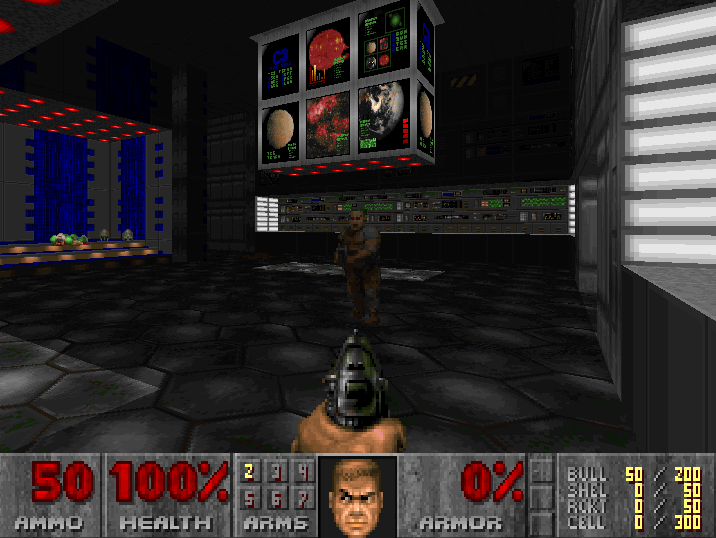
\includegraphics[scale=0.7]{doom.png}
\caption{Screenshot of Doom}
\label{fig:doom}
\end{figure}

%%Czy opisać każdą z pozostałych gier/omawiać konkretny powód jej odrzucenia?
%%Omówić tablę w tekście? Jeśli tak to w jaki sposób - omówić wszystkie wymienione w tabeli kryteria i powody ich wprowadzenia?
%%Tabela jest oparta na wielu źródłach. Jak to przedstawić w pracy?
%%Czy przypisy w komórkach tabeli są akceptowalne? Jeśli nie to w jaki sposób objaśnić zawartość komórki (np. wskazać na istnienie GZDooma korzystającego z OpenGL do renderowania)?  


Lack of scripting support and unaccessible screen buffer were considered as critical factors for rejecting such game and accessing engine's logic only by SDK was considered as a major drawback.
Some of the criteria could not be addressed in form of the statement, becouse they were based on analysis of engine's code in the context of internal architecture and easiness of modification.
Multi-threaded or client-server architecture would make difficult to fully control speed of execution. 


ZDoom based Doom met most of given requirements and allowed to implement features that would by hard or impossible to achieve in other games eg. offscreen rendering and reward computation.
Although Doom wasn't greatly used in research on reinforcement learning, it's recognizability exceeds Unreal Tournament brand.
Originally Doom was designed to work in 320x240 resolution and even so modern implementation allow bigger resolutions, it still utilizes same low resolution textures and rendering algorithm what makes it perfect for generating small visual input data (320x240 or smaller) for reinforcement learning algorithm.
Code analysis showed that access to game logic should be easy, as it is not object-oriented code.
Unique Doom's feature is software renderer. Because of that it could be used without desktop environment (eg. remotely over ssh).
Doom's gameplay is quite simple compared to newer FPS games as it consists mostly of running around and shooting and possible actions could be easly translated for reinforcement learning needs. 
\begin{table}[]
\centering
\caption{Overview of 3D FPS games considered as base of VIZIA environment}
\label{tab:engines}
\begin{tabular}{|r||p{1.3cm}|p{1.3cm}|p{1.3cm}|p{1.3cm}|p{1.3cm}|p{1.3cm}|p{1.3cm}|}
\hline
Game                      & Quake III: Arena & Doom  & Doom 3    & Half-Life 2 & Unreal Tournament 2004 & Unreal Tournament & Cube        \\ \hline
Game Engine               & ioquake3         & zdoom & id tech 4 & Source      & Unreal Engine 2        & Unreal Engine 4   & Cube Engine \\ \hline
Relase year               & 1999             & 1993  & 2003      & 2004        & 2004                   & 2016              & 2001        \\ \hline
Open Source               & \OK              & \OK   & \OK       &             &                        & \OK               & \OK         \\ \hline
Licence                   & GPLv2            & GPL   & GPLv3     & Closed      & Closed                 & Custom            & ZLIB        \\ \hline
Language                  & C                & C++   & C++       & C++         & C++                    & C++               & C++         \\ \hline
DirectX                   &                  &       &           & \OK         &                        & \OK               &             \\ \hline
OpenGL                    & \OK              & \OK   & \OK       & \OK         & \OK                    & \OK               & \OK         \\ \hline
Software Render           &                  & \OK   &           &             &                        &                   &             \\ \hline
Windows                   & \OK              & \OK   & \OK       & \OK         & \OK                    & \OK               & \OK         \\ \hline
Linux                     & \OK              & \OK   &           & \OK         & \OK                    & \OK               & \OK         \\ \hline
Mac OS                    & \OK              & \OK   & \OK       & \OK         & \OK                    & \OK               &             \\ \hline
Scripting                 &                  & \OK   &           & \OK         & \OK                    & \OK               & \OK         \\ \hline
Custom assets             & \OK              & \OK   & \OK       & \OK         & \OK                    & \OK               & \OK         \\ \hline
Map editor                & \OK              & \OK   & \OK       & \OK         & \OK                    & \OK               & \OK         \\ \hline
Multiplayer               & \OK              & \OK   &           &             & \OK                    & \OK               & \OK         \\ \hline
Engine access             & Code             & Code  & Code      & SDK         & SDK                    & SDK               & Code        \\ \hline
Small resolutions         & \OK              & \OK   & \OK       & \OK         & \OK                    & \OK               & \OK         \\ \hline
Screen access             & \OK              & \OK   & \OK       &             &                        & \OK               & \OK         \\ \hline
RAM                       & \OK              & \OK   & \OK       & \OK         & \OK                    &                   & \OK         \\ \hline
Disk space                & 70MB             & 40MB  & 2GB       & 4,5GB       & 6GB                    & \textgreater10GB  & 35MB        \\ \hline
Code complexity           & 6                & 5     & 8         & NA          & NA                     & 11                & 3           \\ \hline
Brand recognition         & 41,1             & 99    & 99        & 36,6        & 1,2                    & 1,2               & 0,1         \\ \hline
Active community          & \OK              & \OK   & \OK       & \OK         &                        & \OK               &             \\ \hline
Free original assets      &                  &       &           &             &                        & \OK               & \OK         \\ \hline
\end{tabular}
\end{table}




\subsection{Operating System}


Linux has been choosen as a target operating system for this environment.
Compilation tool-chain based on CMake and makefile allowed to automate building process and simplify project configuration.
It's stability makes it perfect platform for a long-term research and the biggest share in supercomputers market~\cite{top500} proves it's computing abilities.


\subsection{Game Controller and API}


The basic module for control over Doom - game controller - was written in C++ with usage of Boost library.
It allowed to use Boost::interprocess library in both ZDoom and game controller, as ZDoom was written in C++, what made connecting game controller and game easier than it would be using low level language on the engine side and high level language for the controller.
Experimental Boost::process library was used for control over Doom process.


Above the controller the higher layer of abstraction was implemented defining Application Programming Interface for intelligent agents modules.
It was also developed in C++ what allowed to provide bindings to Python and Java, with possibility to add another eg. Lua, Julia.


Python API was considered as main way of controlling VIZIA Environment by users.
Bindings were prepared  using Boost::python library.
This language is one of the most popular in data science~\cite{ds_lang} and for phrase: "python machine learning" Google Serach Engine returns over 4.6 Millions results (as at 28.01.2016).
There are many machine learning libraries for Python such as scikit-learn or PyBrain.
Because of that providing fully functional Python API was one of the biggest priorities of this project.


For Java bindings Java Native Interface (JNI) was used.


\subsection{Map Editor and Scripting}


Creation of test environments has been made possible by using tools developed by Doom's community for maps and scripts editing: SLADE 3 and Doom Bulider 2. Those tools utilizes ACC -- compilter for Action Code Script (ACS), language, which is supported in ZDoom engine.
This topic was discussed further in Chapter~\ref{ch:scenarios}.

\section{Architecture}
Nice diagram (in DOOM style) with the arcitecture.
\begin{itemize}
\item Zdoom separate process.
\item Boost interprocess: shared memory to comunicate with zdoom.
\item Flow control and PLAYER vs SPECTATOR mode.
\item Warnings and exceptions.
\end{itemize}

\section{Problems and Solutions}
\begin{itemize}
\item Why shared memory and separate doom process and what it entails.
\item Why make/set action are like they are. Why action is a vector not just number.
\item Why state is copied in Python but not in cpp.
\item Zbuffer struggles.
\item Why Windows and Mac are not supported so well.
\item Why scenario is effectively divided into config file nad doom iwad file.
\item Why multiplayer is barely usable.
\end{itemize}

\section{Performance}
Table with some fps ratings and a graph.
Conclusions: it's fast enough, any reasonably good AI will be much slower during learning process.



